\documentclass{article}

\usepackage[utf8]{inputenc}
\usepackage[a4paper, margin=1in]{geometry}
\usepackage{graphicx}

\pagenumbering{gobble}

\title{C\# Code Snippet}
\author{
	Sudhanshu Kumar\\
	2017IEN43\\
	Department of Computer Science
}

\begin{document}
	\maketitle
	\break
	\section*{GUI to check IP address of a host}
	
	\begin{verbatim}
	using System;
	using System.Windows.Forms;
	using System.Net;
	
	namespace hostIP
	{
	public partial class Form1 : Form
	{
	public Form1()
	{
	InitializeComponent();
	}
	
	private void button1_Click(object sender, EventArgs e)
	{
	try
	{
	IPHostEntry hostname = Dns.GetHostByName(textBox1.Text);
	IPAddress[] ip = hostname.AddressList;
	textBox2.Text = ip[0].ToString();
	}
	catch(Exception ex)
	{
	Console.WriteLine(ex.ToString());
	}
	}
	}
	}
	
	
	\end{verbatim}
	
	\begin{center}
		\textbf{Outputs}\\
		\hfill\break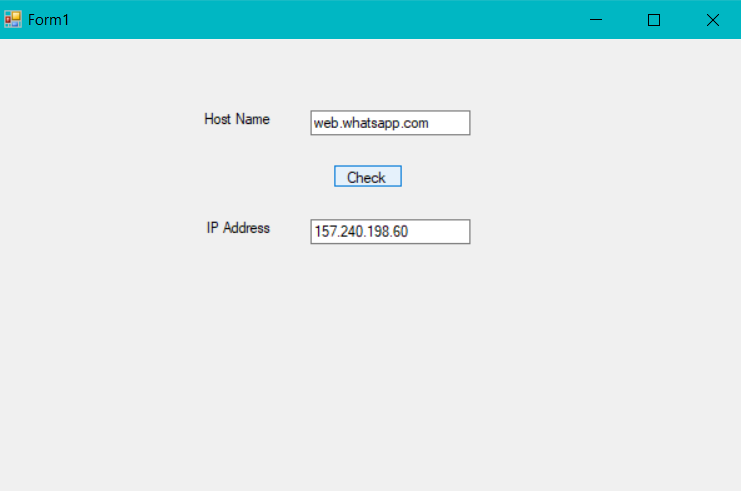
\includegraphics[width=4.27in]{1.png}\\
		\hfill\break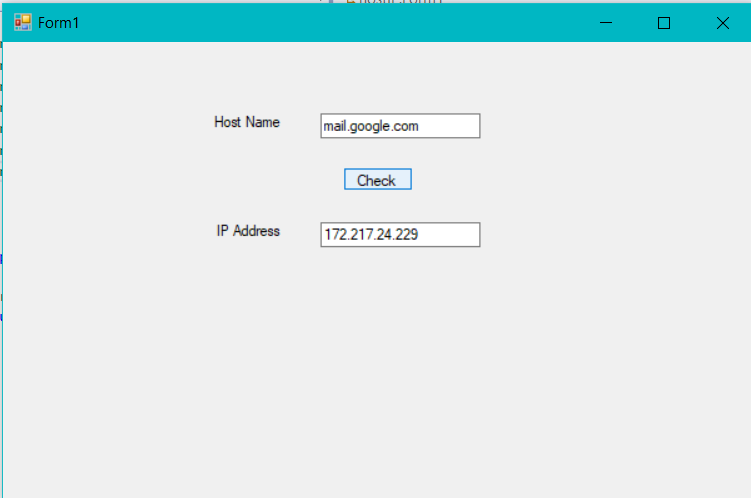
\includegraphics[width=4.27in]{2.png}\\
		\hfill\break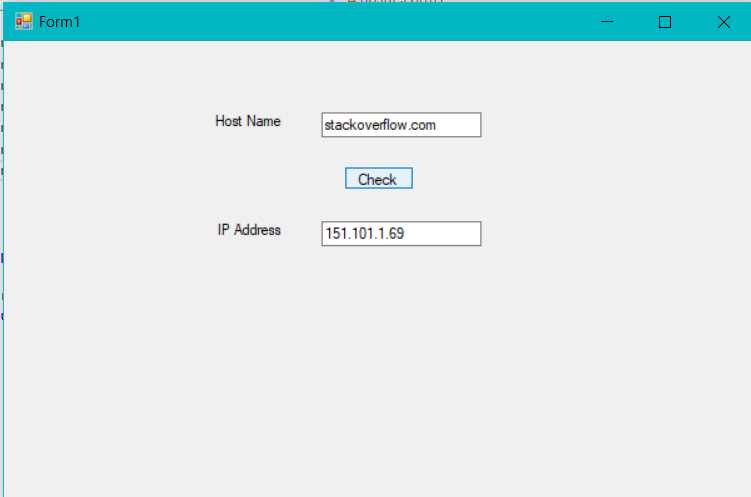
\includegraphics[width=4.27in]{3.png}\\
		\hfill\break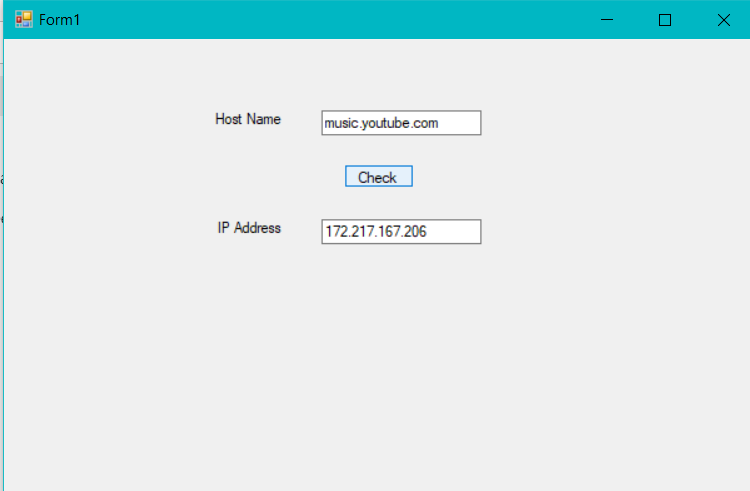
\includegraphics[width=4.27in]{4.png}\\
		\hfill\break\rule{6.27in}{1.2pt}
		\hfill\break\textbf{\emph{Thanks, Stay Hydrated and Keep Breathing.}}
	\end{center}
\end{document}